\documentclass{beamer}
\usepackage[size=a4]{beamerposter}
 
\usepackage{tikz}
\usetikzlibrary{arrows,automata,fit}

\begin{document}

\begin{frame}

\frametitle{Latent dirichlet allocation for classification}
~\\
\textbf{\large{Introduction to document analysis}}~\\
~\\
\begin{itemize}
\item \textbf{Term Frequency-Inverse Document Frequency (tf-idf),}~\\ \textit{Salton and McGill, 1983}~\\
$\rightarrow$ Reduces the arbitrary length documents to a fixed length of numbers~\\
~\\
\item \textbf{Latent semantic indexing}, \textit{Deerwester et al., 1990}~\\
$\rightarrow$ Similar to principal component analysis~\\
$\rightarrow$ Uses decomposition of the tf-idf matrix~\\
$ \rightarrow$ Preserving the most important semantic information~\\
~\\
\item \textbf{Probabilistic Latent Semantic Indexing}, \textit{Hoffmann 1999}~\\
$\rightarrow$ Each word in a document is a sample from a mixture of multinomials~\\
$\rightarrow$The document is represented as a list of mixing proportions.~\\
$\rightarrow$ Limits : no generative model + complexity proportionnal to the size of the corpus
\end{itemize}

\end{frame}

\begin{frame}
\frametitle{Presentation of the LDA model}
%\section*{Presentation of the LDA model}
\begin{figure}
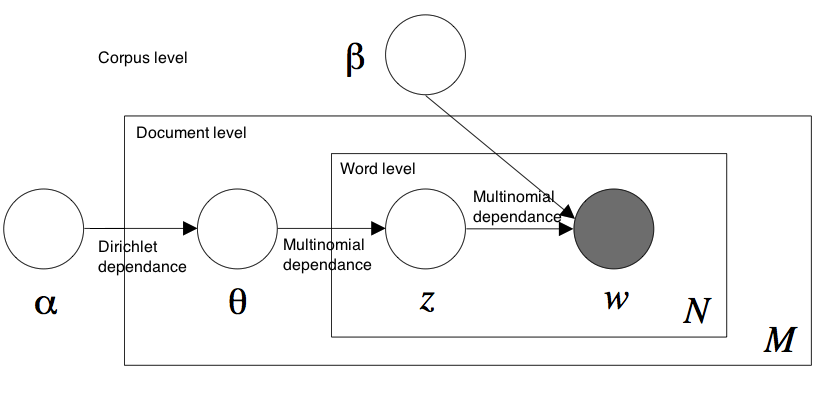
\includegraphics[width=18cm]{LDA}~\\
\end{figure}

$\rightarrow$Different model scales : corpus, document, word.~\\
~\\
$\rightarrow$Main assumption of the model : exchangeability of the documents and words in the document [De Finetti's theorem for the form of distribution]~\\
~\\
$\rightarrow$Procedure for document generation with respect to the graphical model~\\

\end{frame}

\begin{frame}
\frametitle{Presentation of the LDA model}
\begin{figure}
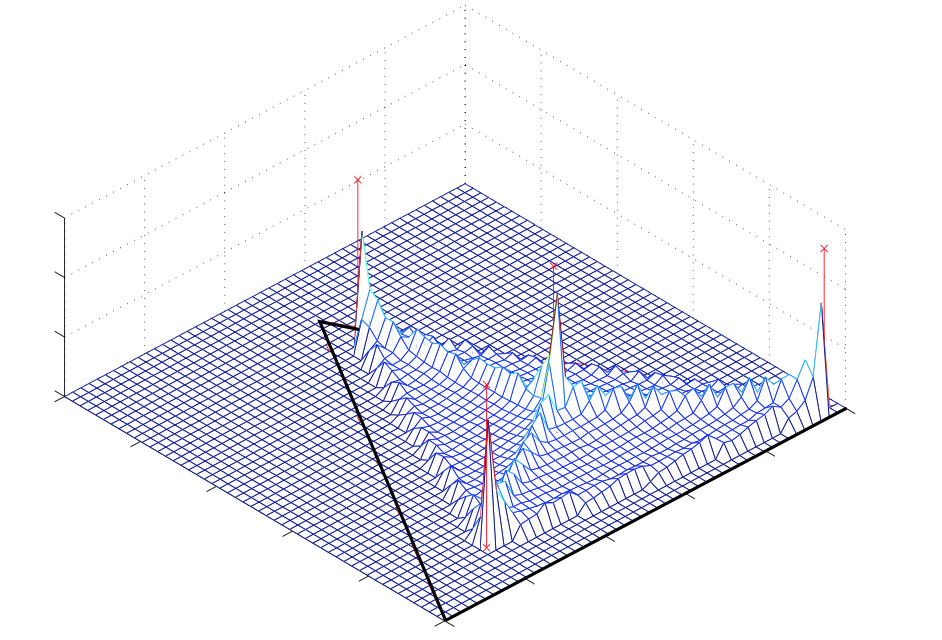
\includegraphics[width=12cm]{Simplex}~\\
\caption{Exemple with $ \theta \in $ 2D simplex }
\end{figure}
%\section*{Presentation of the LDA model}
$\rightarrow$ $\theta$ generates a multinomial topic distribution~\\
~\\
$\rightarrow$ This topic distribution generates words. In the case of 3 words, deterministic distribution on the vertices, midpoint of an edge gives probability 0.5 to two of the words, centroid of the triangle is the uniform distribution over the words~\\
~\\
$\rightarrow$Aim : estimation of corpus parameters $\alpha$ and $\beta$ for agenerative model of $p(\theta,z | \omega, \alpha, \beta)$

\end{frame}



\begin{frame}
\frametitle{Application to document classification}


Classification : 

SVM on posterior Dirichlet parameter gamma associated with the document


\end{frame}

\end{document}